\chapter{चालक और विद्युतरोधी}\label{ch:g4:conductors-insulators}

बिजली के तार धातु के क्यों बनते हैं --- पर उन्हें प्लास्टिक क्यों
पहनाया जाता है? \omterm{ex:g3:first-electric-circuit:switch}{स्विच} का नन्हा पुल धारा क्यों चलाता है, जबकि उसका
खोल तुम्हारी उँगलियों को सुरक्षित रखता है? पिछले साल हमने फंदे बंद
किए थे; इस साल हम पूछते हैं कि बिजली किन-किन पदार्थों में से गुज़र भी
सकती है। उत्तर हर पदार्थ को दो हिस्सों में बाँट देता है: \omterm{def:g4:conductors-insulators:conductor}{चालक} और
\omterm{def:g4:conductors-insulators:insulator}{विद्युतरोधी}।

\section{जाँच-यंत्र}

\begin{method}[जाँच-यंत्र बनाना]\label{met:g4:conductors-insulators:tester}
पिछले साल वाला फंदा बनाओ --- \omterm{def:g3:first-electric-circuit:battery}{बैटरी}, तार, \omterm{def:g3:first-electric-circuit:bulb}{बल्ब} --- पर जान-बूझकर एक
दरार छोड़ दो: दो खुले तार-सिरे, एक उँगली भर की दूरी पर।
\begin{enumerate}
  \item दोनों खुले सिरे आपस में छुआओ: \omterm{def:g3:first-electric-circuit:bulb}{बल्ब} जल उठता है --- जाँच-यंत्र
        काम कर रहा है;
  \item जिस वस्तु की जाँच करनी है उससे दरार पाटो, उसका एक-एक सिरा
        कसकर एक-एक तार से दबाओ;
  \item \omterm{def:g3:first-electric-circuit:bulb}{बल्ब} देखो: जलना यानी बिजली वस्तु के पार निकल गई; अँधेरा यानी
        निकल ही नहीं सकी।
\end{enumerate}
उत्तर \omterm{def:g3:first-electric-circuit:bulb}{बल्ब} देता है: वह ठीक तभी जलता है जब जाँची जा रही वस्तु फंदा पूरा
कर देती है।
\end{method}

\begin{omfigure}
\begin{tikzpicture}[scale=0.9]
  \draw (0,0) to[battery1, l=बैटरी] (0,2.6)
    to[short] (2.2,2.6)
    to[lamp, l=बल्ब] (4.4,2.6)
    to[short] (6.0,2.6) -- (6.0,1.7);
  \draw (6.0,0.9) -- (6.0,0) to[short] (0,0);
  \fill (6.0,1.7) circle (1.6pt) node[right, font=\small]
    {~खुला सिरा};
  \fill (6.0,0.9) circle (1.6pt) node[right, font=\small]
    {~खुला सिरा};
  \draw[thick, fill=omMeth, fill opacity=0.4]
    (5.75,0.95) rectangle (6.25,1.65);
  \node[right, font=\small] at (6.6,1.3) {जाँची जा रही वस्तु};
\end{tikzpicture}

{\small जाँच-यंत्र: एक भला-चंगा फंदा, जिसमें एक दरार है। जो भी उस दरार
को पाटे उसी की जाँच हो रही है --- \omterm{def:g3:first-electric-circuit:bulb}{बल्ब} बता देता है कि धारा उसके पार
जाती है या नहीं।}
\end{omfigure}

\section{चालक और विद्युतरोधी}

\begin{definition}[चालक]\label{def:g4:conductors-insulators:conductor}
\emph{चालक}\index{चालक} वह पदार्थ है जो बिजली को अपने में से गुज़रने
देता है। जाँच-यंत्र में दरार पाटने वाला चालक फंदा बंद कर देता है और
\omterm{def:g3:first-electric-circuit:bulb}{बल्ब} जला देता है।
\end{definition}

\begin{definition}[विद्युतरोधी]\label{def:g4:conductors-insulators:insulator}
\emph{विद्युतरोधी}\index{विद्युतरोधी} वह पदार्थ है जो बिजली को रोक
देता है। विद्युतरोधी से दरार पाटने पर फंदा पहले जितना ही खुला रहता है:
\omterm{def:g3:first-electric-circuit:bulb}{बल्ब} अँधेरा ही रहता है।
\end{definition}

\begin{example}[जाँचों से भरी एक सुबह]\label{ex:g4:conductors-insulators:trials}
कक्षा के जाँच-यंत्र के नतीजे: इस्पात की क्लिप --- \omterm{def:g1:light-and-shadows:source}{प्रकाश}। सिक्का ---
\omterm{def:g1:light-and-shadows:source}{प्रकाश}। रसोई की एल्यूमिनियम पन्नी --- \omterm{def:g1:light-and-shadows:source}{प्रकाश}। चाबी --- \omterm{def:g1:light-and-shadows:source}{प्रकाश}।
प्लास्टिक का रूलर --- अँधेरा। लकड़ी की पेंसिल --- अँधेरा। काँच की
गोली --- अँधेरा। रबर की रबड़ --- अँधेरा। काग़ज़ की पट्टी --- अँधेरा।
पैटर्न ख़ुद उछलकर सामने आ जाता है: \omterm{def:g3:first-electric-circuit:bulb}{बल्ब} जलाने वाली सारी वस्तुएँ धातु
की बनी हैं।
\end{example}

\begin{proposition}[धातुएँ चालक होती हैं]\label{prop:g4:conductors-insulators:metals}
हर धातु बिजली की \omterm{def:g4:conductors-insulators:conductor}{चालक} है --- लोहा, ताँबा, एल्यूमिनियम, सोना, सब की
सब; इसीलिए \omterm{def:g1:magnets:magnet}{चुंबक} का सिर्फ़ लोहे पर अड़ना हमें चौंका गया था, पर
जाँच-यंत्र कभी नहीं चौंकाएगा। रोज़मर्रा के बाक़ी ज़्यादातर \omterm{def:g3:solids-liquids-gases:solid}{ठोस} ---
प्लास्टिक, लकड़ी, काँच, रबर, काग़ज़, मोम --- \omterm{def:g4:conductors-insulators:insulator}{विद्युतरोधी} हैं।
\end{proposition}

\begin{remark}[चालक होना चुंबकीय होना नहीं है]\label{rem:g4:conductors-insulators:notmagnet}
धातु की इन दोनों प्रतिभाओं को आपस में मत मिलाओ। \omterm{def:g1:magnets:magnet}{चुंबक} सिर्फ़ लोहे और
उसके कुनबे को चुनता है; विद्युत धारा कहीं कम नखरे करती है और
\emph{हर} धातु में से गुज़र जाती है। जिस एल्यूमिनियम की पन्नी ने
तुम्हारे \omterm{def:g1:magnets:magnet}{चुंबक} को अनदेखा कर दिया था, वही धारा बहुत अच्छी तरह ले जाती
है --- दो अलग खेल, दो अलग नियम।
\end{remark}

\section{चालक और विद्युतरोधी साथ-साथ काम करते हैं}

\begin{example}[तार की बनावट]\label{ex:g4:conductors-insulators:wire}
लैंप की तार जहाँ प्लग में घुसती है, वहाँ उसका सिरा देखो: भीतर चमकीला
ताँबा चलता है --- \omterm{def:g4:conductors-insulators:conductor}{चालक}, यानी धारा की सड़क; उसके चारों ओर रंगीन
प्लास्टिक लिपटा है --- \omterm{def:g4:conductors-insulators:insulator}{विद्युतरोधी}, यानी सड़क की बाड़। काम ताँबा करता
है; प्लास्टिक धारा को भीतर और तुम्हारी उँगलियों को बाहर रखता है।
तुम्हारे घर की हर केबल इन दोनों की जोड़ी है: \omterm{def:g4:conductors-insulators:insulator}{विद्युतरोधी} के भीतर एक
\omterm{def:g4:conductors-insulators:conductor}{चालक}।
\end{example}

\begin{omfigure}
\begin{tikzpicture}[scale=0.85]
  \draw[thick, fill=omExo, fill opacity=0.25]
    (0.5,0.35) rectangle (6.5,1.65);
  \draw[thick, fill=omThm, fill opacity=0.45]
    (0.5,0.78) rectangle (7.6,1.22);
  \node[right, font=\small] at (8.35,1.8) {प्लास्टिक की परत: विद्युतरोधी};
  \draw[-Stealth, omExo] (8.3,1.8) -- (6.3,1.55);
  \node[right, font=\small] at (8.35,1.0) {ताँबे का क्रोड: चालक};
  \draw[-Stealth, omExo] (8.3,1.0) -- (7.72,1.0);
\end{tikzpicture}

{\small बिजली की केबल, कपड़े उतारकर: धारा के लिए ताँबे की सड़क, और
सुरक्षा के लिए उसके चारों ओर प्लास्टिक की बाड़।}
\end{omfigure}

\begin{omfigure}
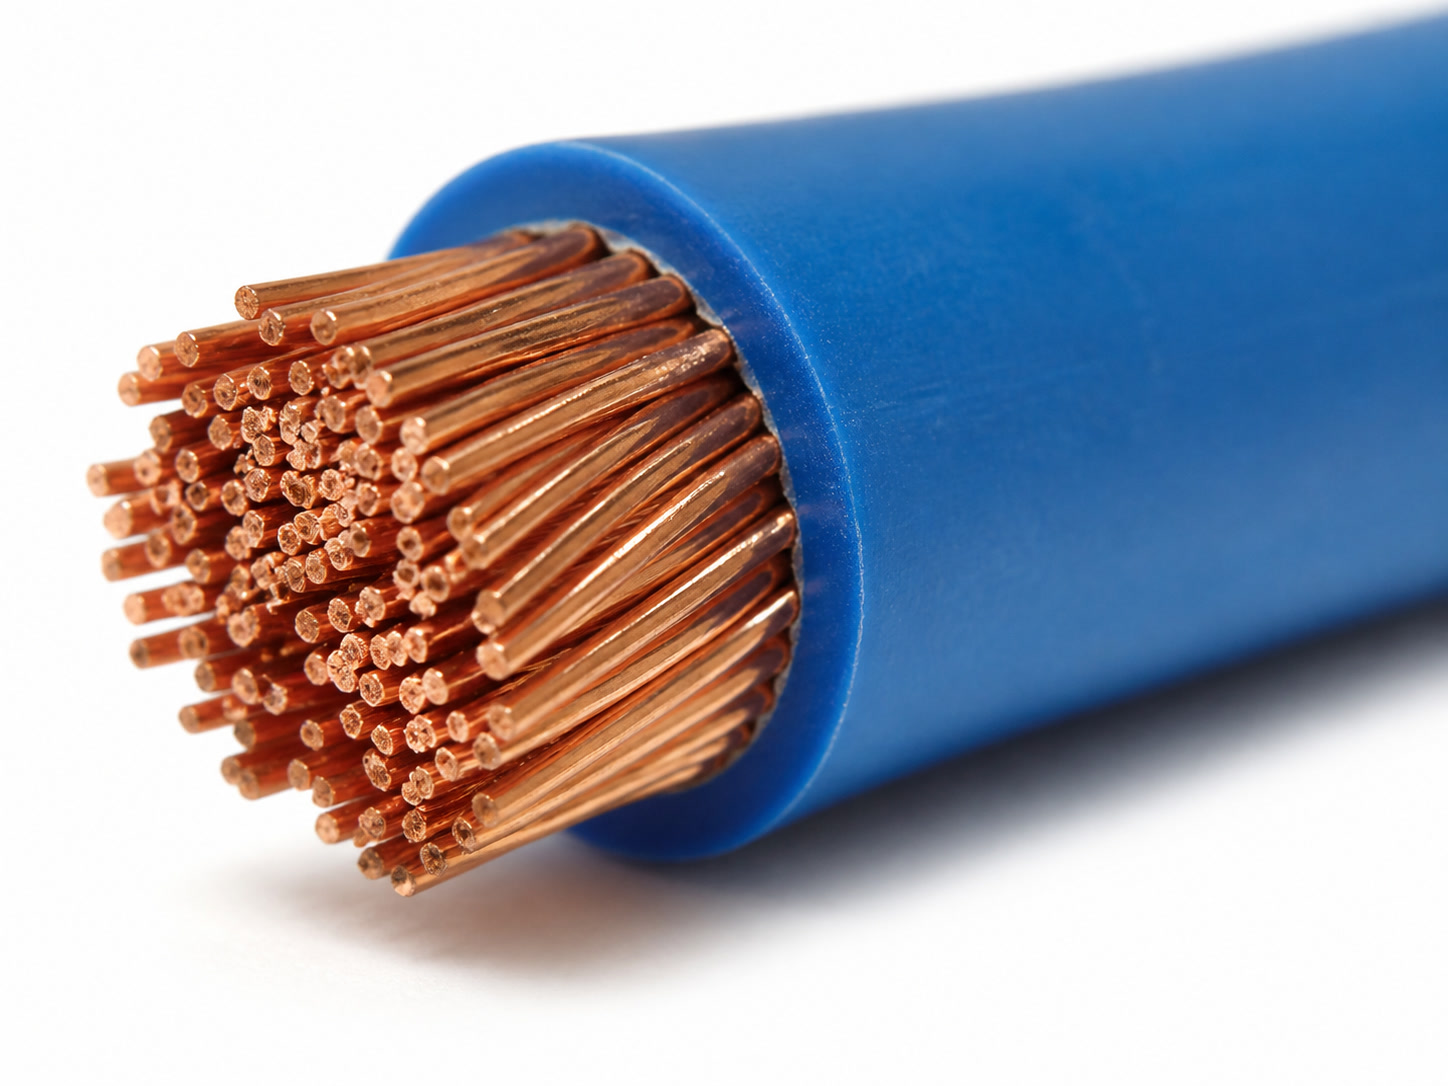
\includegraphics[width=0.5\linewidth]{images/book1/ai/g4-conductors-cable.jpg}

{\small असली केबल का कटा सिरा: रंगीन प्लास्टिक की परत के भीतर ताँबे की चमकीली लड़ें --- यानी \omterm{def:g4:conductors-insulators:insulator}{विद्युतरोधी} के भीतर \omterm{def:g4:conductors-insulators:conductor}{चालक}।}
\end{omfigure}

\begin{example}[रोज़मर्रा की चीज़ें पढ़ना]\label{ex:g4:conductors-insulators:objects}
अब बहुत-सी बनावटें ख़ुद अपनी सफ़ाई दे देती हैं। \omterm{ex:g3:first-electric-circuit:switch}{स्विच}: प्लास्टिक के
खोल में धातु का पुल (पुल को धारा ले जानी है, तुम्हारी उँगली को नहीं)।
बिजली वाले का पेचकस: इस्पात की छड़, और मोटी \omterm{def:g4:conductors-insulators:insulator}{विद्युतरोधी} मूठ। सॉकेट:
भीतर गहराई में धातु, बाहर प्लास्टिक का चेहरा। बिजली के खंभे नंगी धातु
की केबल ऊँचाई पर, हाथ से दूर ले जाते हैं, और उन्हें लंबी \omterm{def:g4:conductors-insulators:insulator}{विद्युतरोधी}
तश्तरियों से लटकाते हैं ताकि धारा खंभे में रिस न जाए।
\end{example}

\begin{remark}[पानी, लोग, और नियम क्यों हैं]\label{rem:g4:conductors-insulators:safety}
एक और \omterm{def:g4:conductors-insulators:conductor}{चालक} का नाम लेना ज़रूरी है: \emph{नम चीज़ें} --- जिनमें नम
मानव त्वचा भी शामिल है। हम बुरे \omterm{def:g4:conductors-insulators:conductor}{चालक} हैं, पर दीवार का सॉकेट इतने
ज़ोर से धकेलता है कि ``बुरा'' भी काफ़ी से ज़्यादा हो जाता है।
सुरक्षा के जो नियम तुम जानते हो, उनकी गहरी वजह यही है: सॉकेट में कभी
कुछ मत घुसाओ, गीले हाथों से बिजली की किसी चीज़ को मत छुओ, और बाल
सुखाने वाले यंत्र नहाने की जगह से दूर रखो। \omterm{def:g3:first-electric-circuit:battery}{बैटरी} वाला जाँच-यंत्र
\emph{इसलिए} सुरक्षित है कि \omterm{def:g3:first-electric-circuit:battery}{बैटरी} का धक्का बहुत हल्का होता है; सॉकेट
किसी को माफ़ नहीं करता।
\end{remark}

\section{अभ्यास}

\begin{exercise}[$\star$]\label{exo:g4:conductors-insulators:1}
\omterm{def:g4:conductors-insulators:conductor}{चालक} क्या है? \omterm{def:g4:conductors-insulators:insulator}{विद्युतरोधी} क्या है? जाँच-यंत्र का \omterm{def:g3:first-electric-circuit:bulb}{बल्ब} इनमें से कौन
जलाता है?
\end{exercise}

\begin{exercise}[$\star$]\label{exo:g4:conductors-insulators:2}
चालकों और विद्युतरोधियों में छाँटो: इस्पात का चम्मच; \ कॉर्क; \
रसोई की पन्नी; \ एक गिलास; \ ताँबे का सिक्का; \ प्लास्टिक का ब्लॉक।
\end{exercise}

\begin{exercise}[$\star$]\label{exo:g4:conductors-insulators:3}
किसी भी जाँच से पहले यह कैसे पक्का करोगे कि ख़ुद जाँच-यंत्र काम कर
रहा है? यह जाँच ज़रूरी क्यों है?
\end{exercise}

\begin{exercise}[$\star$]\label{exo:g4:conductors-insulators:4}
जाँची जा रही किसी वस्तु पर \omterm{def:g3:first-electric-circuit:bulb}{बल्ब} अँधेरा रह जाता है। दो संभव कारण बताओ
--- एक वस्तु के बारे में, एक लापरवाह जाँच के बारे में।
\end{exercise}

\begin{exercise}[$\star$]\label{exo:g4:conductors-insulators:5}
लैंप की केबल भीतर से ताँबे की और बाहर से प्लास्टिक की क्यों होती है?
हर पदार्थ कौन-सा काम करता है?
\end{exercise}

\begin{exercise}[$\star$]\label{exo:g4:conductors-insulators:6}
\omterm{ex:g3:first-electric-circuit:switch}{स्विच} में कौन-सा हिस्सा \omterm{def:g4:conductors-insulators:conductor}{चालक} है और कौन-सा \omterm{def:g4:conductors-insulators:insulator}{विद्युतरोधी}? उसे दोनों
क्यों चाहिए?
\end{exercise}

\begin{exercise}[$\star$]\label{exo:g4:conductors-insulators:7}
एल्यूमिनियम की पन्नी \omterm{def:g1:magnets:magnet}{चुंबक} को पूरी तरह अनदेखा कर देती है। क्या वह
जाँच-यंत्र का \omterm{def:g3:first-electric-circuit:bulb}{बल्ब} जलाएगी? कौन-सा नियम उत्तर देता है, और
\cref{rem:g4:conductors-insulators:notmagnet} किस गड़बड़ी से सावधान
करती है?
\end{exercise}

\begin{exercise}[$\star$]\label{exo:g4:conductors-insulators:8}
पेंसिल लकड़ी की होती है और उसके भीतर ग्रेफ़ाइट की सलाख़। नीनो का
जाँच-यंत्र रंगी हुई लकड़ी पर अँधेरा रहता है, पर छिली हुई ग्रेफ़ाइट
की नोक से नोक तक हल्का-सा जल उठता है। नीनो ने पेंसिल के दोनों
पदार्थों के बारे में क्या खोज निकाला?
\end{exercise}

\begin{exercise}[$\star$]\label{exo:g4:conductors-insulators:9}
बिजली वालों के पेचकस और प्लास की मूठें मोटे प्लास्टिक की क्यों होती
हैं? कौन-सा पदार्थ किसकी रक्षा कर रहा है?
\end{exercise}

\begin{exercise}[$\star\star$]\label{exo:g4:conductors-insulators:10}
जाँच-यंत्र में गले की धातु की ज़ंजीर ``\omterm{def:g1:light-and-shadows:source}{प्रकाश}'' देती है; लकड़ी के
मनकों वाली माला ``अँधेरा''; और मोटे सूती धागे में गाँठ लगाकर पिरोए गए
धातु के मनकों वाली माला भी ``अँधेरा'' --- जबकि हर मनका \omterm{def:g4:conductors-insulators:conductor}{चालक} है!
मनके-दर-मनके धारा की सड़क का पीछा करते हुए तीसरा नतीजा समझाओ।
\end{exercise}

\begin{exercise}[$\star\star$]\label{exo:g4:conductors-insulators:11}
गीले हाथों से बिजली की चीज़ें छूना सूखे हाथों से छूने के मुक़ाबले
कहीं ज़्यादा ख़तरनाक क्यों है? और तुम्हारे प्रयोगों के लिए \omterm{def:g3:first-electric-circuit:battery}{बैटरी} वाला
जाँच-यंत्र सुरक्षित क्यों है, जबकि सॉकेट कभी नहीं?
\cref{rem:g4:conductors-insulators:safety} का उपयोग करो।
\end{exercise}
